\newif\ifsolutions
\solutionstrue % Show solutions
%\solutionsfalse % Hide solutions

\documentclass{article}
\usepackage{geometry}
\geometry{margin=1in}
\usepackage{tikz}
\usepackage{amssymb}

% fleqn allows setting indent of display math
\usepackage[fleqn]{amsmath}
\setlength{\mathindent}{0pt} % Set indent
% Disable equation numbering (https://tex.stackexchange.com/a/360378)
\makeatletter
\renewcommand\tagform@[1]{}
\makeatother

% Allow Unicode (some, e.g., © and £ at least)
% https://tex.stackexchange.com/questions/370278/is-there-any-reason-to-use-inputenc
\usepackage[utf8]{inputenc}

% Hyperlinks
\usepackage{hyperref}
\hypersetup{colorlinks=true, urlcolor=blue, linkcolor=blue}

% Prevent indentation of paragraphs
\setlength\parindent{0pt}
\setlength{\parskip}{\baselineskip}

% Spacing above/below equations
% https://tex.stackexchange.com/a/69678
\AtBeginDocument{%
 \abovedisplayskip=-\parskip
 \abovedisplayshortskip=-\parskip
 \belowdisplayskip=0pt
 \belowdisplayshortskip=0pt
}

% Allow 3 additional subsection levels
% https://tex.stackexchange.com/a/60212
\usepackage{titlesec}
\setcounter{secnumdepth}{6}
% H4 in HTML
\titleformat{\paragraph}{\normalfont\normalsize\bfseries}{\theparagraph}{1em}{}
\titlespacing*{\paragraph}{0pt}{3.25ex plus 1ex minus .2ex}{1.5ex plus .2ex}
% H5 in HTML
\titleformat{\subparagraph}{\normalfont\normalsize\bfseries}{\thesubparagraph}{1em}{}
\titlespacing*{\subparagraph}{0pt}{3.25ex plus 1ex minus .2ex}{1.5ex plus .2ex}
% H6 in HTML
\titleformat{\subsubparagraph}{\normalfont\normalsize\bfseries}{\thesubsubparagraph}{1em}{}
\titlespacing*{\subsubparagraph}{0pt}{3.25ex plus 1ex minus .2ex}{1.5ex plus .2ex}

% So enumerate at all levels is numbers
% https://tex.stackexchange.com/questions/78842/nested-enumeration-numbering
\renewcommand{\labelenumii}{\arabic{enumii}.}
\renewcommand{\labelenumiii}{\arabic{enumiii}.}
\renewcommand{\labelenumiv}{\arabic{enumiv}.}

\renewcommand{\mbox}{\text}
\newcommand{\ds}[0]{\displaystyle}
\newcommand{\ihat}[0]{\hat{\boldsymbol{\imath}}}
\newcommand{\jhat}[0]{\hat{\boldsymbol{\jmath}}}
\newcommand{\khat}[0]{\hat{\boldsymbol{k}}}
\newcommand{\xhat}[0]{\hat{\mathbf{x}}}
\newcommand{\yhat}[0]{\hat{\mathbf{y}}}
\newcommand{\zhat}[0]{\hat{\mathbf{z}}}
\newcommand{\rhat}[0]{\hat{\mathbf{r}}}
\newcommand{\bfvec}[1]{\vec{\mathbf{#1}}}
\newcommand{\bfcdot}[0]{\boldsymbol{\cdot}}

\usepackage{fancyhdr}
\pagestyle{fancy}
\lhead{Capacitance}
\rhead{\thepage}
\fancyfoot{}

\begin{document}

\section{Overview}

\subsection{Technique}

The general technique for computing capacitance when Gauss's law applies is:

\begin{enumerate}

  \item Place an equal and opposite amount of charge, $Q$, on the conductors.

  \item Use Gauss's law to compute the electric field between the conductors.

  \item Use $V(b)-V(a)=-\int^b_a \mathbf{E}\bfcdot d\mathbf{l}$ to find the potential difference between the conductors.

  \item Use the equation for capacitance to find $C$: $C = Q/|\Delta V| = Q/|V(b)-V(a)|$.

\end{enumerate}

\subsection{Review of Related Topics}

\textbf{Conductors}

\begin{enumerate}

  \item When charges are placed on an isolated conductor (meaning it is far away from other charges), they will reconfigure themselves to make the electric field inside the conductor zero.

  \item If a charged conductor is not isolated, the charges on the conductor will reconfigure themselves to make the electric field inside the conductor zero. The total field in the conductor is the field due to the charges on the conductor and charges elsewhere.

\end{enumerate}

\textbf{Electric Potential Energy and Electric Potential}

The general formula for work is $W_{a\rightarrow b}=\int_a^b \bfvec{F}\bfcdot d\bfvec{l}$. If $\bfvec{F}$ is a conservative force, such as the force due to a static electric field, we define potential energy $U$ according to

$\Delta U = U(b)-U(a) \equiv -W_{a\rightarrow b}$

The force on a charge $q_o$ in an electric field $\bfvec{E}$ is $\bfvec{F}=q_o\bfvec{E}$ and so we can write

$\ds U(b)-U(a) = -\int_a^b q_o\bfvec{E}\bfcdot d\bfvec{l}$. Dividing both sides by $q_o$ gives $\ds\frac{U(b)}{q_o}-\frac{U(a)}{q_o} = -\int_a^b\bfvec{E}\bfcdot d\bfvec{l}$

Defining electric potential as $V\equiv U/q_o$ gives $V(b)-V(a) = -\int_a^b\bfvec{E}\bfcdot d\bfvec{l}$

In summary, if you calculate the difference in potential between $a$ and $b$ (in Volts), you can also determine, for a charge $q_o$ moved from $a$ to $b$,

\begin{enumerate}

  \item how much work (in Joules) the electric field did on the charge: $-q_o(V(b)-V(a))$, and

  \item the change in the charge's electric potential energy (in Joules): $+q_o(V(b)-V(a))$.

\end{enumerate}

\ifsolutions\else
\newpage
\fi

\section{Parallel Plates}

An equal and opposite amount of charge is placed on two conducting and parallel plates, as shown on the left in the following figure. On the right, a side view of the plates is shown. The area of the plates, $A = w^2$, is much larger than shown, such that the width, $w$, is much larger than the separation distance, $d$.



\tikzset{every picture/.style={line width=0.75pt}} %set default line width to 0.75pt        

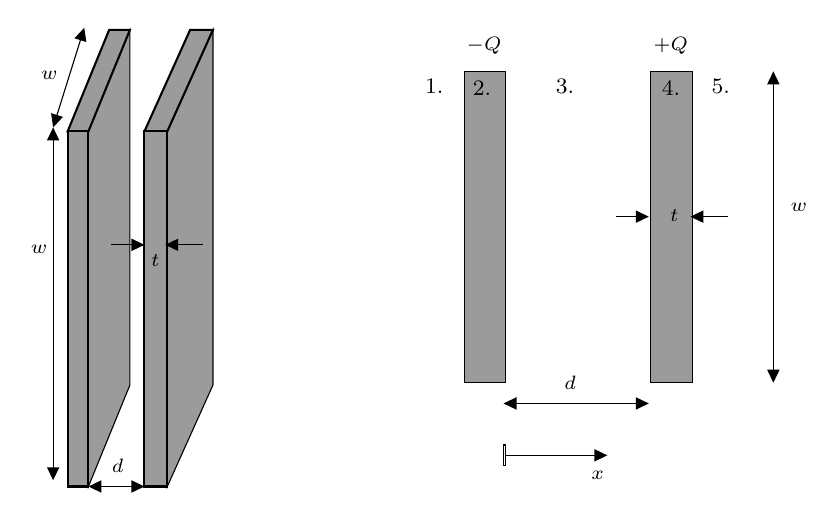
\begin{tikzpicture}[x=0.75pt,y=0.75pt,yscale=-1,xscale=1]
%uncomment if require: \path (0,238); %set diagram left start at 0, and has height of 238

%Shape: Rectangle [id:dp4781425563552617] 
\draw  [color={rgb, 255:red, 0; green, 0; blue, 0 }  ,draw opacity=1 ][fill={rgb, 255:red, 155; green, 155; blue, 155 }  ,fill opacity=1 ] (221,30) -- (241,30) -- (241,180) -- (221,180) -- cycle ;
%Shape: Rectangle [id:dp6627321392123502] 
\draw  [color={rgb, 255:red, 0; green, 0; blue, 0 }  ,draw opacity=1 ][fill={rgb, 255:red, 155; green, 155; blue, 155 }  ,fill opacity=1 ] (311,30) -- (331,30) -- (331,180) -- (311,180) -- cycle ;
%Straight Lines [id:da050416454278339407] 
\draw    (243,190) -- (307,190) ;
\draw [shift={(310,190)}, rotate = 180] [fill={rgb, 255:red, 0; green, 0; blue, 0 }  ][line width=0.08]  [draw opacity=0] (6.25,-3) -- (0,0) -- (6.25,3) -- cycle    ;
\draw [shift={(240,190)}, rotate = 0] [fill={rgb, 255:red, 0; green, 0; blue, 0 }  ][line width=0.08]  [draw opacity=0] (6.25,-3) -- (0,0) -- (6.25,3) -- cycle    ;
%Straight Lines [id:da669587499539398] 
\draw    (43,230) -- (64,230) ;
\draw [shift={(67,230)}, rotate = 180] [fill={rgb, 255:red, 0; green, 0; blue, 0 }  ][line width=0.08]  [draw opacity=0] (6.25,-3) -- (0,0) -- (6.25,3) -- cycle    ;
\draw [shift={(40,230)}, rotate = 0] [fill={rgb, 255:red, 0; green, 0; blue, 0 }  ][line width=0.08]  [draw opacity=0] (6.25,-3) -- (0,0) -- (6.25,3) -- cycle    ;
%Shape: Polygon [id:ds48793909345474673] 
\draw  [draw opacity=0][fill={rgb, 255:red, 155; green, 155; blue, 155 }  ,fill opacity=1 ][line width=1.5]  (50,10) -- (50,181.11) -- (30,230) -- (30,58.89) -- cycle ;
%Shape: Polygon [id:ds9808941595699727] 
\draw  [color={rgb, 255:red, 0; green, 0; blue, 0 }  ,draw opacity=1 ][fill={rgb, 255:red, 155; green, 155; blue, 155 }  ,fill opacity=1 ] (60,10) -- (60,181.11) -- (40,230) -- (40,58.89) -- cycle ;
%Shape: Polygon [id:ds7281613636786879] 
\draw  [color={rgb, 255:red, 0; green, 0; blue, 0 }  ,draw opacity=1 ][fill={rgb, 255:red, 155; green, 155; blue, 155 }  ,fill opacity=1 ][line width=0.75]  (60,10) -- (40,58.89) -- (30,58.89) -- (50,10) -- cycle ;
%Shape: Polygon [id:ds010997684504611582] 
\draw  [color={rgb, 255:red, 0; green, 0; blue, 0 }  ,draw opacity=1 ][fill={rgb, 255:red, 155; green, 155; blue, 155 }  ,fill opacity=1 ][line width=0.75]  (40,58.89) -- (40,230) -- (30,230) -- (30,58.89) -- cycle ;

%Straight Lines [id:da2244240649960263] 
\draw    (23.89,54.14) -- (37.11,11.86) ;
\draw [shift={(38,9)}, rotate = 107.35] [fill={rgb, 255:red, 0; green, 0; blue, 0 }  ][line width=0.08]  [draw opacity=0] (6.25,-3) -- (0,0) -- (6.25,3) -- cycle    ;
\draw [shift={(23,57)}, rotate = 287.35] [fill={rgb, 255:red, 0; green, 0; blue, 0 }  ][line width=0.08]  [draw opacity=0] (6.25,-3) -- (0,0) -- (6.25,3) -- cycle    ;
%Straight Lines [id:da7344448006041042] 
\draw    (23,60) -- (23,224) ;
\draw [shift={(23,227)}, rotate = 270] [fill={rgb, 255:red, 0; green, 0; blue, 0 }  ][line width=0.08]  [draw opacity=0] (6.25,-3) -- (0,0) -- (6.25,3) -- cycle    ;
\draw [shift={(23,57)}, rotate = 90] [fill={rgb, 255:red, 0; green, 0; blue, 0 }  ][line width=0.08]  [draw opacity=0] (6.25,-3) -- (0,0) -- (6.25,3) -- cycle    ;
%Shape: Rectangle [id:dp5380194246766798] 
\draw   (240,210) -- (241,210) -- (241,220) -- (240,220) -- cycle ;
%Straight Lines [id:da057592777072014156] 
\draw    (240.5,215) -- (287,215) ;
\draw [shift={(290,215)}, rotate = 180] [fill={rgb, 255:red, 0; green, 0; blue, 0 }  ][line width=0.08]  [draw opacity=0] (6.25,-3) -- (0,0) -- (6.25,3) -- cycle    ;
%Shape: Polygon [id:ds9492933425452903] 
\draw  [draw opacity=0][fill={rgb, 255:red, 155; green, 155; blue, 155 }  ,fill opacity=1 ][line width=1.5]  (89,10) -- (89,181.11) -- (67,230) -- (67,58.89) -- cycle ;
%Shape: Polygon [id:ds46227237706637814] 
\draw  [color={rgb, 255:red, 0; green, 0; blue, 0 }  ,draw opacity=1 ][fill={rgb, 255:red, 155; green, 155; blue, 155 }  ,fill opacity=1 ] (100,10) -- (100,181.11) -- (78,230) -- (78,58.89) -- cycle ;
%Shape: Polygon [id:ds16834684381886045] 
\draw  [color={rgb, 255:red, 0; green, 0; blue, 0 }  ,draw opacity=1 ][fill={rgb, 255:red, 155; green, 155; blue, 155 }  ,fill opacity=1 ][line width=0.75]  (100,10) -- (78,58.89) -- (67,58.89) -- (89,10) -- cycle ;
%Shape: Polygon [id:ds6208970266098528] 
\draw  [color={rgb, 255:red, 0; green, 0; blue, 0 }  ,draw opacity=1 ][fill={rgb, 255:red, 155; green, 155; blue, 155 }  ,fill opacity=1 ][line width=0.75]  (78,58.89) -- (78,230) -- (67,230) -- (67,58.89) -- cycle ;

%Straight Lines [id:da304858444201656] 
\draw    (51,113.57) -- (64,113.57) ;
\draw [shift={(67,113.57)}, rotate = 180] [fill={rgb, 255:red, 0; green, 0; blue, 0 }  ][line width=0.08]  [draw opacity=0] (6.25,-3) -- (0,0) -- (6.25,3) -- cycle    ;
%Straight Lines [id:da022134641801796473] 
\draw    (95,113.57) -- (80,113.57) ;
\draw [shift={(77,113.57)}, rotate = 360] [fill={rgb, 255:red, 0; green, 0; blue, 0 }  ][line width=0.08]  [draw opacity=0] (6.25,-3) -- (0,0) -- (6.25,3) -- cycle    ;
%Straight Lines [id:da9216205628160365] 
\draw    (370,33) -- (370,177) ;
\draw [shift={(370,180)}, rotate = 270] [fill={rgb, 255:red, 0; green, 0; blue, 0 }  ][line width=0.08]  [draw opacity=0] (6.25,-3) -- (0,0) -- (6.25,3) -- cycle    ;
\draw [shift={(370,30)}, rotate = 90] [fill={rgb, 255:red, 0; green, 0; blue, 0 }  ][line width=0.08]  [draw opacity=0] (6.25,-3) -- (0,0) -- (6.25,3) -- cycle    ;
%Straight Lines [id:da8606516356050204] 
\draw    (348,100) -- (333,100) ;
\draw [shift={(330,100)}, rotate = 360] [fill={rgb, 255:red, 0; green, 0; blue, 0 }  ][line width=0.08]  [draw opacity=0] (6.25,-3) -- (0,0) -- (6.25,3) -- cycle    ;
%Straight Lines [id:da8775319862635156] 
\draw    (294,100) -- (307,100) ;
\draw [shift={(310,100)}, rotate = 180] [fill={rgb, 255:red, 0; green, 0; blue, 0 }  ][line width=0.08]  [draw opacity=0] (6.25,-3) -- (0,0) -- (6.25,3) -- cycle    ;

% Text Node
\draw (311,12.4) node [anchor=north west][inner sep=0.75pt]  [font=\scriptsize]  {$+Q$};
% Text Node
\draw (221,12.4) node [anchor=north west][inner sep=0.75pt]  [font=\scriptsize]  {$-Q$};
% Text Node
\draw (268,175.4) node [anchor=north west][inner sep=0.75pt]  [font=\scriptsize]  {$d$};
% Text Node
\draw (224,33.4) node [anchor=north west][inner sep=0.75pt]  [font=\footnotesize]  {$2.$};
% Text Node
\draw (201,32.4) node [anchor=north west][inner sep=0.75pt]  [font=\footnotesize]  {$1.$};
% Text Node
\draw (264,32.4) node [anchor=north west][inner sep=0.75pt]  [font=\footnotesize]  {$3.$};
% Text Node
\draw (315,33.4) node [anchor=north west][inner sep=0.75pt]  [font=\footnotesize]  {$4.$};
% Text Node
\draw (339,32.4) node [anchor=north west][inner sep=0.75pt]  [font=\footnotesize]  {$5.$};
% Text Node
\draw (281,221.4) node [anchor=north west][inner sep=0.75pt]  [font=\scriptsize]  {$x$};
% Text Node
\draw (50,215.4) node [anchor=north west][inner sep=0.75pt]  [font=\scriptsize]  {$d$};
% Text Node
\draw (16,28.4) node [anchor=north west][inner sep=0.75pt]  [font=\scriptsize]  {$w$};
% Text Node
\draw (11,112.4) node [anchor=north west][inner sep=0.75pt]  [font=\scriptsize]  {$w$};
% Text Node
\draw (69,116.97) node [anchor=north west][inner sep=0.75pt]  [font=\scriptsize]  {$t$};
% Text Node
\draw (377,92.4) node [anchor=north west][inner sep=0.75pt]  [font=\scriptsize]  {$w$};
% Text Node
\draw (319,95.4) node [anchor=north west][inner sep=0.75pt]  [font=\scriptsize]  {$t$};


\end{tikzpicture}


\begin{enumerate}

  \item How will the charges distribute on each of the plates? That is, how much charge is on each of the four faces that have an area $A$? Assume that no charge appears on the other (thin, and having thickness $t$) faces of the plates, which have a much smaller area.

     \ifsolutions
       {\bf Answer}: The charges will move to the inner faces, as shown in the following diagram. Electric field vectors for the positive and negative charges are shown. Because the charges are on a large plane, the field is independent of distance from the plane. With this charge configuration, inside the conductors, the field due to the positive charges cancels the field due to the negative charges giving a net field of zero.

       

\tikzset{every picture/.style={line width=0.75pt}} %set default line width to 0.75pt        

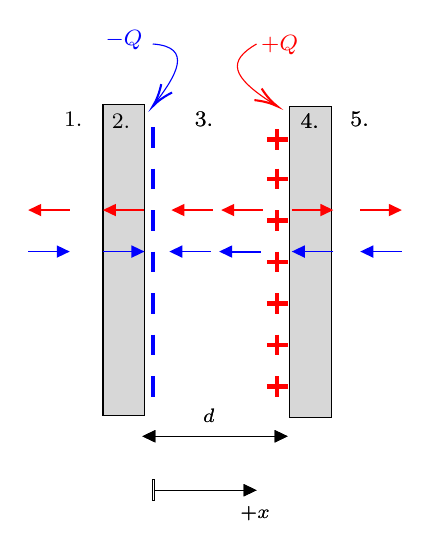
\begin{tikzpicture}[x=0.75pt,y=0.75pt,yscale=-1,xscale=1]
%uncomment if require: \path (0,255); %set diagram left start at 0, and has height of 255

%Shape: Rectangle [id:dp4275263890544876] 
\draw  [color={rgb, 255:red, 0; green, 0; blue, 0 }  ,draw opacity=1 ][fill={rgb, 255:red, 155; green, 155; blue, 155 }  ,fill opacity=0.4 ] (136,50) -- (156,50) -- (156,200) -- (136,200) -- cycle ;
%Shape: Rectangle [id:dp9533247951265795] 
\draw  [color={rgb, 255:red, 0; green, 0; blue, 0 }  ,draw opacity=1 ][fill={rgb, 255:red, 155; green, 155; blue, 155 }  ,fill opacity=0.4 ] (46,49) -- (66,49) -- (66,199) -- (46,199) -- cycle ;
%Straight Lines [id:da6139754077056814] 
\draw    (68,209) -- (132,209) ;
\draw [shift={(135,209)}, rotate = 180] [fill={rgb, 255:red, 0; green, 0; blue, 0 }  ][line width=0.08]  [draw opacity=0] (6.25,-3) -- (0,0) -- (6.25,3) -- cycle    ;
\draw [shift={(65,209)}, rotate = 0] [fill={rgb, 255:red, 0; green, 0; blue, 0 }  ][line width=0.08]  [draw opacity=0] (6.25,-3) -- (0,0) -- (6.25,3) -- cycle    ;
%Shape: Rectangle [id:dp1605497897718935] 
\draw   (70,230) -- (71,230) -- (71,240) -- (70,240) -- cycle ;
%Straight Lines [id:da37406717797821387] 
\draw    (70.5,235) -- (117,235) ;
\draw [shift={(120,235)}, rotate = 180] [fill={rgb, 255:red, 0; green, 0; blue, 0 }  ][line width=0.08]  [draw opacity=0] (6.25,-3) -- (0,0) -- (6.25,3) -- cycle    ;
%Shape: Rectangle [id:dp7304091212122024] 
\draw  [color={rgb, 255:red, 0; green, 0; blue, 0 }  ,draw opacity=1 ] (46,49) -- (66,49) -- (66,199) -- (46,199) -- cycle ;
%Straight Lines [id:da33949359685304326] 
\draw    (68,209) -- (132,209) ;
\draw [shift={(135,209)}, rotate = 180] [fill={rgb, 255:red, 0; green, 0; blue, 0 }  ][line width=0.08]  [draw opacity=0] (6.25,-3) -- (0,0) -- (6.25,3) -- cycle    ;
\draw [shift={(65,209)}, rotate = 0] [fill={rgb, 255:red, 0; green, 0; blue, 0 }  ][line width=0.08]  [draw opacity=0] (6.25,-3) -- (0,0) -- (6.25,3) -- cycle    ;
%Shape: Rectangle [id:dp25610705349634855] 
\draw   (70,230) -- (71,230) -- (71,240) -- (70,240) -- cycle ;
%Straight Lines [id:da4375417714391101] 
\draw    (70.5,235) -- (117,235) ;
\draw [shift={(120,235)}, rotate = 180] [fill={rgb, 255:red, 0; green, 0; blue, 0 }  ][line width=0.08]  [draw opacity=0] (6.25,-3) -- (0,0) -- (6.25,3) -- cycle    ;
%Straight Lines [id:da22593772796529743] 
\draw [color={rgb, 255:red, 255; green, 0; blue, 0 }  ,draw opacity=1 ]   (99,100) -- (82,100) ;
\draw [shift={(79,100)}, rotate = 360] [fill={rgb, 255:red, 255; green, 0; blue, 0 }  ,fill opacity=1 ][line width=0.08]  [draw opacity=0] (6.25,-3) -- (0,0) -- (6.25,3) -- cycle    ;
%Straight Lines [id:da9166780279465419] 
\draw [color={rgb, 255:red, 255; green, 0; blue, 0 }  ,draw opacity=1 ]   (137,100) -- (154,100) ;
\draw [shift={(157,100)}, rotate = 180] [fill={rgb, 255:red, 255; green, 0; blue, 0 }  ,fill opacity=1 ][line width=0.08]  [draw opacity=0] (6.25,-3) -- (0,0) -- (6.25,3) -- cycle    ;
%Straight Lines [id:da38697775473150164] 
\draw [color={rgb, 255:red, 255; green, 0; blue, 0 }  ,draw opacity=1 ]   (170,100) -- (187,100) ;
\draw [shift={(190,100)}, rotate = 180] [fill={rgb, 255:red, 255; green, 0; blue, 0 }  ,fill opacity=1 ][line width=0.08]  [draw opacity=0] (6.25,-3) -- (0,0) -- (6.25,3) -- cycle    ;
%Straight Lines [id:da40781377342806824] 
\draw [color={rgb, 255:red, 255; green, 0; blue, 0 }  ,draw opacity=1 ]   (66,100) -- (49,100) ;
\draw [shift={(46,100)}, rotate = 360] [fill={rgb, 255:red, 255; green, 0; blue, 0 }  ,fill opacity=1 ][line width=0.08]  [draw opacity=0] (6.25,-3) -- (0,0) -- (6.25,3) -- cycle    ;
%Straight Lines [id:da21919729719928238] 
\draw [color={rgb, 255:red, 255; green, 0; blue, 0 }  ,draw opacity=1 ]   (30,100) -- (13,100) ;
\draw [shift={(10,100)}, rotate = 360] [fill={rgb, 255:red, 255; green, 0; blue, 0 }  ,fill opacity=1 ][line width=0.08]  [draw opacity=0] (6.25,-3) -- (0,0) -- (6.25,3) -- cycle    ;
%Straight Lines [id:da3828385111314101] 
\draw [color={rgb, 255:red, 0; green, 0; blue, 255 }  ,draw opacity=1 ]   (10,120) -- (27,120) ;
\draw [shift={(30,120)}, rotate = 180] [fill={rgb, 255:red, 0; green, 0; blue, 255 }  ,fill opacity=1 ][line width=0.08]  [draw opacity=0] (6.25,-3) -- (0,0) -- (6.25,3) -- cycle    ;
%Straight Lines [id:da2716728595852598] 
\draw [color={rgb, 255:red, 0; green, 0; blue, 255 }  ,draw opacity=1 ]   (46,120) -- (63,120) ;
\draw [shift={(66,120)}, rotate = 180] [fill={rgb, 255:red, 0; green, 0; blue, 255 }  ,fill opacity=1 ][line width=0.08]  [draw opacity=0] (6.25,-3) -- (0,0) -- (6.25,3) -- cycle    ;
%Straight Lines [id:da654604971455772] 
\draw [color={rgb, 255:red, 0; green, 0; blue, 255 }  ,draw opacity=1 ]   (98,120) -- (81,120) ;
\draw [shift={(78,120)}, rotate = 360] [fill={rgb, 255:red, 0; green, 0; blue, 255 }  ,fill opacity=1 ][line width=0.08]  [draw opacity=0] (6.25,-3) -- (0,0) -- (6.25,3) -- cycle    ;
%Straight Lines [id:da45311004757081164] 
\draw [color={rgb, 255:red, 0; green, 0; blue, 255 }  ,draw opacity=1 ]   (157,120) -- (140,120) ;
\draw [shift={(137,120)}, rotate = 360] [fill={rgb, 255:red, 0; green, 0; blue, 255 }  ,fill opacity=1 ][line width=0.08]  [draw opacity=0] (6.25,-3) -- (0,0) -- (6.25,3) -- cycle    ;
%Straight Lines [id:da04703043046437272] 
\draw [color={rgb, 255:red, 0; green, 0; blue, 255 }  ,draw opacity=1 ]   (190,120) -- (173,120) ;
\draw [shift={(170,120)}, rotate = 360] [fill={rgb, 255:red, 0; green, 0; blue, 255 }  ,fill opacity=1 ][line width=0.08]  [draw opacity=0] (6.25,-3) -- (0,0) -- (6.25,3) -- cycle    ;
%Curve Lines [id:da12711553252246555] 
\draw [color={rgb, 255:red, 0; green, 0; blue, 255 }  ,draw opacity=1 ]   (70,20) .. controls (89.8,21.37) and (81.18,35.39) .. (71.1,48.57) ;
\draw [shift={(70,50)}, rotate = 307.75] [color={rgb, 255:red, 0; green, 0; blue, 255 }  ,draw opacity=1 ][line width=0.75]    (10.93,-3.29) .. controls (6.95,-1.4) and (3.31,-0.3) .. (0,0) .. controls (3.31,0.3) and (6.95,1.4) .. (10.93,3.29)   ;
%Curve Lines [id:da224561224684787] 
\draw [color={rgb, 255:red, 255; green, 0; blue, 0 }  ,draw opacity=1 ]   (120,20) .. controls (105.88,28.21) and (107.41,35.67) .. (128.35,48.97) ;
\draw [shift={(130,50)}, rotate = 211.8] [color={rgb, 255:red, 255; green, 0; blue, 0 }  ,draw opacity=1 ][line width=0.75]    (10.93,-3.29) .. controls (6.95,-1.4) and (3.31,-0.3) .. (0,0) .. controls (3.31,0.3) and (6.95,1.4) .. (10.93,3.29)   ;
%Straight Lines [id:da9826207023497178] 
\draw [color={rgb, 255:red, 0; green, 0; blue, 255 }  ,draw opacity=1 ][line width=0.75]    (122,120) -- (105,120) ;
\draw [shift={(102,120)}, rotate = 360] [fill={rgb, 255:red, 0; green, 0; blue, 255 }  ,fill opacity=1 ][line width=0.08]  [draw opacity=0] (6.25,-3) -- (0,0) -- (6.25,3) -- cycle    ;
%Straight Lines [id:da6600078838091041] 
\draw [color={rgb, 255:red, 255; green, 0; blue, 0 }  ,draw opacity=1 ][line width=0.75]    (123,100) -- (106,100) ;
\draw [shift={(103,100)}, rotate = 360] [fill={rgb, 255:red, 255; green, 0; blue, 0 }  ,fill opacity=1 ][line width=0.08]  [draw opacity=0] (6.25,-3) -- (0,0) -- (6.25,3) -- cycle    ;
%Straight Lines [id:da49730767878081994] 
\draw [color={rgb, 255:red, 0; green, 0; blue, 255 }  ,draw opacity=1 ][line width=1.5]    (70,60) -- (70,70) ;
%Straight Lines [id:da1564998625144418] 
\draw [color={rgb, 255:red, 0; green, 0; blue, 255 }  ,draw opacity=1 ][line width=1.5]    (70,80) -- (70,90) ;
%Straight Lines [id:da7742983779891199] 
\draw [color={rgb, 255:red, 0; green, 0; blue, 255 }  ,draw opacity=1 ][line width=1.5]    (70,100) -- (70,110) ;
%Straight Lines [id:da4312646986493218] 
\draw [color={rgb, 255:red, 0; green, 0; blue, 255 }  ,draw opacity=1 ][line width=1.5]    (70,120) -- (70,130) ;
%Straight Lines [id:da312538381836716] 
\draw [color={rgb, 255:red, 0; green, 0; blue, 255 }  ,draw opacity=1 ][line width=1.5]    (70,140) -- (70,150) ;
%Straight Lines [id:da7404419797973874] 
\draw [color={rgb, 255:red, 0; green, 0; blue, 255 }  ,draw opacity=1 ][line width=1.5]    (70,160) -- (70,170) ;
%Straight Lines [id:da2427617105037123] 
\draw [color={rgb, 255:red, 0; green, 0; blue, 255 }  ,draw opacity=1 ][line width=1.5]    (70,180) -- (70,190) ;
%Straight Lines [id:da9629786560212747] 
\draw [color={rgb, 255:red, 255; green, 0; blue, 0 }  ,draw opacity=1 ][line width=1.5]    (130,61) -- (130,71) ;
%Straight Lines [id:da09158335617758406] 
\draw [color={rgb, 255:red, 255; green, 0; blue, 0 }  ,draw opacity=1 ][line width=1.5]    (125,66) -- (135,66) ;
%Straight Lines [id:da8433361305275593] 
\draw [color={rgb, 255:red, 255; green, 0; blue, 0 }  ,draw opacity=1 ][line width=1.5]    (130,80) -- (130,90) ;
%Straight Lines [id:da1085760422813713] 
\draw [color={rgb, 255:red, 255; green, 0; blue, 0 }  ,draw opacity=1 ][line width=1.5]    (125,85) -- (135,85) ;
%Straight Lines [id:da5118687521443328] 
\draw [color={rgb, 255:red, 255; green, 0; blue, 0 }  ,draw opacity=1 ][line width=1.5]    (130,100) -- (130,110) ;
%Straight Lines [id:da904877245142782] 
\draw [color={rgb, 255:red, 255; green, 0; blue, 0 }  ,draw opacity=1 ][line width=1.5]    (125,105) -- (135,105) ;
%Straight Lines [id:da3682621991783923] 
\draw [color={rgb, 255:red, 255; green, 0; blue, 0 }  ,draw opacity=1 ][line width=1.5]    (130,120) -- (130,130) ;
%Straight Lines [id:da04827305196457843] 
\draw [color={rgb, 255:red, 255; green, 0; blue, 0 }  ,draw opacity=1 ][line width=1.5]    (125,125) -- (135,125) ;
%Straight Lines [id:da4707800348275146] 
\draw [color={rgb, 255:red, 255; green, 0; blue, 0 }  ,draw opacity=1 ][line width=1.5]    (130,140) -- (130,150) ;
%Straight Lines [id:da19072213957683282] 
\draw [color={rgb, 255:red, 255; green, 0; blue, 0 }  ,draw opacity=1 ][line width=1.5]    (125,145) -- (135,145) ;
%Straight Lines [id:da1209798262835613] 
\draw [color={rgb, 255:red, 255; green, 0; blue, 0 }  ,draw opacity=1 ][line width=1.5]    (130,160) -- (130,170) ;
%Straight Lines [id:da07445338235417354] 
\draw [color={rgb, 255:red, 255; green, 0; blue, 0 }  ,draw opacity=1 ][line width=1.5]    (125,165) -- (135,165) ;
%Straight Lines [id:da5912104373246556] 
\draw [color={rgb, 255:red, 255; green, 0; blue, 0 }  ,draw opacity=1 ][line width=1.5]    (130,180) -- (130,190) ;
%Straight Lines [id:da1741940568923046] 
\draw [color={rgb, 255:red, 255; green, 0; blue, 0 }  ,draw opacity=1 ][line width=1.5]    (125,185) -- (135,185) ;

% Text Node
\draw (46,12.4) node [anchor=north west][inner sep=0.75pt]  [font=\footnotesize]  {$\textcolor[rgb]{0,0,1}{-Q}$};
% Text Node
\draw (93,194.4) node [anchor=north west][inner sep=0.75pt]  [font=\scriptsize]  {$d$};
% Text Node
\draw (49,52.4) node [anchor=north west][inner sep=0.75pt]  [font=\footnotesize]  {$2.$};
% Text Node
\draw (26,51.4) node [anchor=north west][inner sep=0.75pt]  [font=\footnotesize]  {$1.$};
% Text Node
\draw (89,51.4) node [anchor=north west][inner sep=0.75pt]  [font=\footnotesize]  {$3.$};
% Text Node
\draw (140,52.4) node [anchor=north west][inner sep=0.75pt]  [font=\footnotesize]  {$4.$};
% Text Node
\draw (164,51.4) node [anchor=north west][inner sep=0.75pt]  [font=\footnotesize]  {$5.$};
% Text Node
\draw (111,241.4) node [anchor=north west][inner sep=0.75pt]  [font=\scriptsize]  {$+x$};
% Text Node
\draw (121,14.4) node [anchor=north west][inner sep=0.75pt]  [font=\footnotesize,color={rgb, 255:red, 255; green, 0; blue, 0 }  ,opacity=1 ]  {$+Q$};
% Text Node
\draw (93,194.4) node [anchor=north west][inner sep=0.75pt]  [font=\scriptsize]  {$d$};
% Text Node
\draw (89,51.4) node [anchor=north west][inner sep=0.75pt]  [font=\footnotesize]  {$3.$};
% Text Node
\draw (140,52.4) node [anchor=north west][inner sep=0.75pt]  [font=\footnotesize]  {$4.$};
% Text Node
\draw (164,51.4) node [anchor=north west][inner sep=0.75pt]  [font=\footnotesize]  {$5.$};
% Text Node
\draw (111,241.4) node [anchor=north west][inner sep=0.75pt]  [font=\scriptsize]  {$+x$};


\end{tikzpicture}

     \else
       \vskip 36pt
     \fi
     \ifsolutions\else
     \vskip 36pt
     \fi

  \item What is the electric field in each of the five regions? (Hint: The magnitude of the field due to charges uniformly distributed on a plane is $|\sigma|/2\epsilon_o$. The field in each region will be the sum of the field due to charges on each plate. Your answer should be such that the electric field inside the conducting plates is zero!)

     \ifsolutions
       {\bf Answer}: The magnitude of the field due to each charged surface is $|\sigma|/2\epsilon_o$, where $\sigma$ is the surface charge density. The surface charge densities are $\pm Q/A$.  

       

\tikzset{every picture/.style={line width=0.75pt}} %set default line width to 0.75pt        

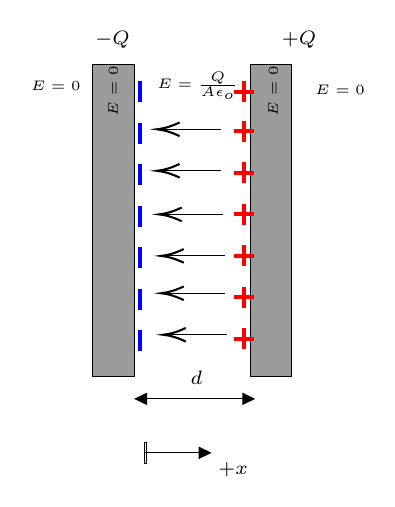
\begin{tikzpicture}[x=0.75pt,y=0.75pt,yscale=-1,xscale=1]
%uncomment if require: \path (0,245); %set diagram left start at 0, and has height of 245

%Shape: Rectangle [id:dp9057598036648726] 
\draw  [color={rgb, 255:red, 0; green, 0; blue, 0 }  ,draw opacity=1 ][fill={rgb, 255:red, 155; green, 155; blue, 155 }  ,fill opacity=1 ] (60,29.01) -- (80,29.01) -- (80,179.01) -- (60,179.01) -- cycle ;
%Shape: Rectangle [id:dp9855644776713539] 
\draw  [color={rgb, 255:red, 0; green, 0; blue, 0 }  ,draw opacity=1 ][fill={rgb, 255:red, 155; green, 155; blue, 155 }  ,fill opacity=1 ] (136,29.01) -- (156,29.01) -- (156,179.01) -- (136,179.01) -- cycle ;
%Straight Lines [id:da7193616198968829] 
\draw    (122,60.1) -- (93,60.1) ;
\draw [shift={(91,60.1)}, rotate = 360] [color={rgb, 255:red, 0; green, 0; blue, 0 }  ][line width=0.75]    (10.93,-3.29) .. controls (6.95,-1.4) and (3.31,-0.3) .. (0,0) .. controls (3.31,0.3) and (6.95,1.4) .. (10.93,3.29)   ;
%Straight Lines [id:da00958553239241966] 
\draw    (122,80.1) -- (93,80.1) ;
\draw [shift={(91,80.1)}, rotate = 360] [color={rgb, 255:red, 0; green, 0; blue, 0 }  ][line width=0.75]    (10.93,-3.29) .. controls (6.95,-1.4) and (3.31,-0.3) .. (0,0) .. controls (3.31,0.3) and (6.95,1.4) .. (10.93,3.29)   ;
%Straight Lines [id:da010193314753433658] 
\draw    (123,101.1) -- (94,101.1) ;
\draw [shift={(92,101.1)}, rotate = 360] [color={rgb, 255:red, 0; green, 0; blue, 0 }  ][line width=0.75]    (10.93,-3.29) .. controls (6.95,-1.4) and (3.31,-0.3) .. (0,0) .. controls (3.31,0.3) and (6.95,1.4) .. (10.93,3.29)   ;
%Straight Lines [id:da7445084743379691] 
\draw    (124,121.1) -- (95,121.1) ;
\draw [shift={(93,121.1)}, rotate = 360] [color={rgb, 255:red, 0; green, 0; blue, 0 }  ][line width=0.75]    (10.93,-3.29) .. controls (6.95,-1.4) and (3.31,-0.3) .. (0,0) .. controls (3.31,0.3) and (6.95,1.4) .. (10.93,3.29)   ;
%Straight Lines [id:da7169700914802788] 
\draw    (124,139.1) -- (95,139.1) ;
\draw [shift={(93,139.1)}, rotate = 360] [color={rgb, 255:red, 0; green, 0; blue, 0 }  ][line width=0.75]    (10.93,-3.29) .. controls (6.95,-1.4) and (3.31,-0.3) .. (0,0) .. controls (3.31,0.3) and (6.95,1.4) .. (10.93,3.29)   ;
%Straight Lines [id:da849451758154703] 
\draw    (125,159.1) -- (96,159.1) ;
\draw [shift={(94,159.1)}, rotate = 360] [color={rgb, 255:red, 0; green, 0; blue, 0 }  ][line width=0.75]    (10.93,-3.29) .. controls (6.95,-1.4) and (3.31,-0.3) .. (0,0) .. controls (3.31,0.3) and (6.95,1.4) .. (10.93,3.29)   ;
%Straight Lines [id:da35350003303071675] 
\draw [color={rgb, 255:red, 255; green, 0; blue, 0 }  ,draw opacity=1 ][line width=1.5]    (133,37.01) -- (133,47.01) ;
%Straight Lines [id:da18749686188831305] 
\draw [color={rgb, 255:red, 255; green, 0; blue, 0 }  ,draw opacity=1 ][line width=1.5]    (128,42.01) -- (138,42.01) ;
%Straight Lines [id:da899514814843599] 
\draw [color={rgb, 255:red, 255; green, 0; blue, 0 }  ,draw opacity=1 ][line width=1.5]    (133,56.01) -- (133,66.01) ;
%Straight Lines [id:da35479364133898206] 
\draw [color={rgb, 255:red, 255; green, 0; blue, 0 }  ,draw opacity=1 ][line width=1.5]    (128,61.01) -- (138,61.01) ;
%Straight Lines [id:da5994061408121905] 
\draw [color={rgb, 255:red, 255; green, 0; blue, 0 }  ,draw opacity=1 ][line width=1.5]    (133,76.01) -- (133,86.01) ;
%Straight Lines [id:da025011393136393556] 
\draw [color={rgb, 255:red, 255; green, 0; blue, 0 }  ,draw opacity=1 ][line width=1.5]    (128,81.01) -- (138,81.01) ;
%Straight Lines [id:da7250777662474519] 
\draw [color={rgb, 255:red, 255; green, 0; blue, 0 }  ,draw opacity=1 ][line width=1.5]    (133,96.01) -- (133,106.01) ;
%Straight Lines [id:da8024334249013161] 
\draw [color={rgb, 255:red, 255; green, 0; blue, 0 }  ,draw opacity=1 ][line width=1.5]    (128,101.01) -- (138,101.01) ;
%Straight Lines [id:da312935250313392] 
\draw [color={rgb, 255:red, 255; green, 0; blue, 0 }  ,draw opacity=1 ][line width=1.5]    (133,116.01) -- (133,126.01) ;
%Straight Lines [id:da7586150612989309] 
\draw [color={rgb, 255:red, 255; green, 0; blue, 0 }  ,draw opacity=1 ][line width=1.5]    (128,121.01) -- (138,121.01) ;
%Straight Lines [id:da5176838742022054] 
\draw [color={rgb, 255:red, 255; green, 0; blue, 0 }  ,draw opacity=1 ][line width=1.5]    (133,136.01) -- (133,146.01) ;
%Straight Lines [id:da5391062259159898] 
\draw [color={rgb, 255:red, 255; green, 0; blue, 0 }  ,draw opacity=1 ][line width=1.5]    (128,141.01) -- (138,141.01) ;
%Straight Lines [id:da9360148762837004] 
\draw [color={rgb, 255:red, 255; green, 0; blue, 0 }  ,draw opacity=1 ][line width=1.5]    (133,156.01) -- (133,166.01) ;
%Straight Lines [id:da9330433063581276] 
\draw [color={rgb, 255:red, 255; green, 0; blue, 0 }  ,draw opacity=1 ][line width=1.5]    (128,161.01) -- (138,161.01) ;
%Straight Lines [id:da0792673924290197] 
\draw [color={rgb, 255:red, 0; green, 0; blue, 255 }  ,draw opacity=1 ][line width=1.5]    (83,37.01) -- (83,47.01) ;
%Straight Lines [id:da9210352978438316] 
\draw [color={rgb, 255:red, 0; green, 0; blue, 255 }  ,draw opacity=1 ][line width=1.5]    (83,57.01) -- (83,67.01) ;
%Straight Lines [id:da938725717282167] 
\draw [color={rgb, 255:red, 0; green, 0; blue, 255 }  ,draw opacity=1 ][line width=1.5]    (83,77.01) -- (83,87.01) ;
%Straight Lines [id:da7855779912843162] 
\draw [color={rgb, 255:red, 0; green, 0; blue, 255 }  ,draw opacity=1 ][line width=1.5]    (83,97.01) -- (83,107.01) ;
%Straight Lines [id:da9609162568621108] 
\draw [color={rgb, 255:red, 0; green, 0; blue, 255 }  ,draw opacity=1 ][line width=1.5]    (83,117.01) -- (83,127.01) ;
%Straight Lines [id:da6354348204604128] 
\draw [color={rgb, 255:red, 0; green, 0; blue, 255 }  ,draw opacity=1 ][line width=1.5]    (83,137.01) -- (83,147.01) ;
%Straight Lines [id:da46808363520767227] 
\draw [color={rgb, 255:red, 0; green, 0; blue, 255 }  ,draw opacity=1 ][line width=1.5]    (83,157.01) -- (83,167.01) ;
%Shape: Rectangle [id:dp5411815492592136] 
\draw   (85,210.98) -- (86,210.98) -- (86,220.98) -- (85,220.98) -- cycle ;
%Straight Lines [id:da7432245165602127] 
\draw    (83,189.98) -- (135.38,189.98) ;
\draw [shift={(138.38,189.98)}, rotate = 180] [fill={rgb, 255:red, 0; green, 0; blue, 0 }  ][line width=0.08]  [draw opacity=0] (6.25,-3) -- (0,0) -- (6.25,3) -- cycle    ;
\draw [shift={(80,189.98)}, rotate = 0] [fill={rgb, 255:red, 0; green, 0; blue, 0 }  ][line width=0.08]  [draw opacity=0] (6.25,-3) -- (0,0) -- (6.25,3) -- cycle    ;
%Shape: Rectangle [id:dp6472110819276424] 
\draw   (85,210.98) -- (86,210.98) -- (86,220.98) -- (85,220.98) -- cycle ;
%Straight Lines [id:da049120556329296905] 
\draw    (85.5,215.98) -- (114.38,215.98) ;
\draw [shift={(117.38,215.98)}, rotate = 180] [fill={rgb, 255:red, 0; green, 0; blue, 0 }  ][line width=0.08]  [draw opacity=0] (6.25,-3) -- (0,0) -- (6.25,3) -- cycle    ;

% Text Node
\draw (150,11.41) node [anchor=north west][inner sep=0.75pt]  [font=\scriptsize]  {$+Q$};
% Text Node
\draw (60,11.41) node [anchor=north west][inner sep=0.75pt]  [font=\scriptsize]  {$-Q$};
% Text Node
\draw (90,31.41) node [anchor=north west][inner sep=0.75pt]  [font=\tiny]  {$E=\frac{Q}{A\epsilon _{o}}$};
% Text Node
\draw (166,37.41) node [anchor=north west][inner sep=0.75pt]  [font=\tiny]  {$E=0$};
% Text Node
\draw (29,35.41) node [anchor=north west][inner sep=0.75pt]  [font=\tiny]  {$E=0$};
% Text Node
\draw (66.4,55.01) node [anchor=north west][inner sep=0.75pt]  [font=\tiny,rotate=-270]  {$E=0$};
% Text Node
\draw (143.4,55.01) node [anchor=north west][inner sep=0.75pt]  [font=\tiny,rotate=-270]  {$E=0$};
% Text Node
\draw (106,175.38) node [anchor=north west][inner sep=0.75pt]  [font=\scriptsize]  {$d$};
% Text Node
\draw (119.38,219.38) node [anchor=north west][inner sep=0.75pt]  [font=\scriptsize]  {$+x$};


\end{tikzpicture}


       From the diagram in the answer to part 1., the electric fields cancel except between the plates where it is 

       $\ds\frac{|+Q/A|}{2\epsilon_o} + \frac{|-Q/A|}{2\epsilon_o} = \frac{Q}{A\epsilon_o}$

       to the left, so

       $\ds\bfvec{E}=-\frac{Q}{A\epsilon_o}\ihat$
     \else
       \vskip 36pt
     \fi
     \ifsolutions\else
     \vskip 36pt
     \fi

  \item What is the electric potential difference, $V(d)-V(0)$, between the left and right plate? (Make sure the sign of your result matches your expectation based on the techniques covered in the last activity.)

     \ifsolutions
       {\bf Answer}: The general equation is

       $\ds V(b)-V(a) = -\int_a^b\bfvec{E}\bfcdot d\bfvec{l}$

       where $b$ is the final position and $a$ is the initial position. Using our variables,

       $\ds V(d)-V(0) = -\int_0^d\bfvec{E}\bfcdot d\bfvec{l}$

       The electric field is constant, and in the same direction as $x$, so we know the result of the integration will be $\pm Ed=\pm Qd/A\epsilon_o$. Based on techniques covered in the last activity, we expect the potential to be higher at the right plate, so we choose the $+$ option. More formally,

       Using $d\mathbf{l}=dx\ihat$  and $\bfvec{E}=-\frac{Q}{A\epsilon_o}\ihat$ gives

       $\ds V(d)-V(0) = -\int_0^d\bfvec{E}\bfcdot d\bfvec{l}=-\int_0^d\left[-\frac{Q}{A\epsilon_o}\ihat\right]\bfcdot dx\ihat=\frac{Qd}{A\epsilon_o}$
     \else
       \vskip 36pt
     \fi
     \ifsolutions\else
     \vskip 36pt
     \fi

  \item Use your answer to 3. to find the capacitance in terms of $k$, $A$, and $d$.

     \ifsolutions
       {\bf Answer}:

       \begin{equation}
     C = \frac{Q}{|\Delta V|} = \frac{Q}{\frac{Qd}{A\epsilon_o}}=\frac{\epsilon_oA}{d}
     \end{equation}
     \else
       \vskip 36pt
     \fi
     \ifsolutions\else
     \vskip 36pt
     \fi

  \item (Review question) How much work would the electric field do on a charge $q_o$ that is moved from the left plate to the right plate? What would be the change in $q_o$'s electric potential energy?

     \ifsolutions
       {\bf Answer}: $\ds W=-q_o\frac{\epsilon_oA}{d}$. Sign check: The force of the field is to the left and the displacement is to the right, so $\bfvec{F}\bfcdot d\bfvec{l}$ will be negative.

       $\ds\Delta U=-W=q_o\frac{\epsilon_oA}{d}$
     \else
       \vskip 36pt
     \fi
     \ifsolutions\else
     \vskip 36pt
     \fi

\end{enumerate}

\section{Spherical}

Charge placed on two spherical conducting shells, the cross--section of which is shown. Both shells have a thickness of $t$. The inner shell has an outer radius of $a$ and a net charge of $-Q$. The outer shell has an inner radius of $b$ and a net charge of $+Q$. Assume that $Q$ is positive.



\tikzset{every picture/.style={line width=0.75pt}} %set default line width to 0.75pt        

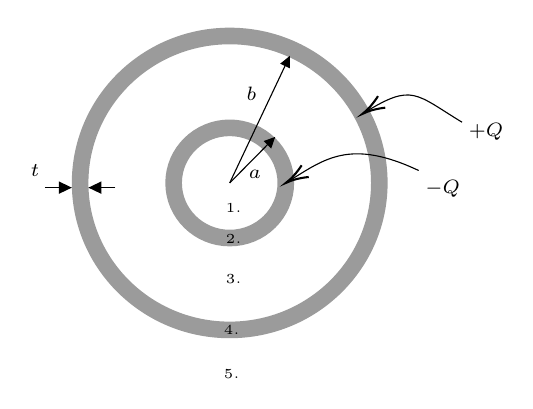
\begin{tikzpicture}[x=0.75pt,y=0.75pt,yscale=-1,xscale=1]
%uncomment if require: \path (0,185); %set diagram left start at 0, and has height of 185

%Shape: Ellipse [id:dp786923384871064] 
\draw  [color={rgb, 255:red, 155; green, 155; blue, 155 }  ,draw opacity=1 ][line width=6]  (36,82.74) .. controls (36,43.63) and (68.27,11.93) .. (108.07,11.93) .. controls (147.88,11.93) and (180.15,43.63) .. (180.15,82.74) .. controls (180.15,121.84) and (147.88,153.55) .. (108.07,153.55) .. controls (68.27,153.55) and (36,121.84) .. (36,82.74) -- cycle ;
%Shape: Ellipse [id:dp7642544577323118] 
\draw  [color={rgb, 255:red, 155; green, 155; blue, 155 }  ,draw opacity=1 ][line width=6]  (81.05,82.74) .. controls (81.05,68.07) and (93.15,56.18) .. (108.07,56.18) .. controls (123,56.18) and (135.1,68.07) .. (135.1,82.74) .. controls (135.1,97.4) and (123,109.29) .. (108.07,109.29) .. controls (93.15,109.29) and (81.05,97.4) .. (81.05,82.74) -- cycle ;
%Straight Lines [id:da023238427542429108] 
\draw    (108.07,82.74) -- (127.89,62.68) ;
\draw [shift={(130,60.55)}, rotate = 134.66] [fill={rgb, 255:red, 0; green, 0; blue, 0 }  ][line width=0.08]  [draw opacity=0] (5.36,-2.57) -- (0,0) -- (5.36,2.57) -- cycle    ;
%Straight Lines [id:da026482910185540165] 
\draw    (108.07,82.74) -- (135.72,24.26) ;
\draw [shift={(137,21.55)}, rotate = 115.3] [fill={rgb, 255:red, 0; green, 0; blue, 0 }  ][line width=0.08]  [draw opacity=0] (5.36,-2.57) -- (0,0) -- (5.36,2.57) -- cycle    ;
%Straight Lines [id:da8792066435104271] 
\draw    (53,85) -- (43,85) ;
\draw [shift={(40,85)}, rotate = 360] [fill={rgb, 255:red, 0; green, 0; blue, 0 }  ][line width=0.08]  [draw opacity=0] (6.25,-3) -- (0,0) -- (6.25,3) -- cycle    ;
%Straight Lines [id:da5223957758570585] 
\draw    (19,85) -- (29,85) ;
\draw [shift={(32,85)}, rotate = 180] [fill={rgb, 255:red, 0; green, 0; blue, 0 }  ][line width=0.08]  [draw opacity=0] (6.25,-3) -- (0,0) -- (6.25,3) -- cycle    ;
%Curve Lines [id:da0374365538769168] 
\draw    (199.1,76.74) .. controls (166.12,61.22) and (153.84,71.14) .. (136.71,81.75) ;
\draw [shift={(135.1,82.74)}, rotate = 328.68] [color={rgb, 255:red, 0; green, 0; blue, 0 }  ][line width=0.75]    (10.93,-3.29) .. controls (6.95,-1.4) and (3.31,-0.3) .. (0,0) .. controls (3.31,0.3) and (6.95,1.4) .. (10.93,3.29)   ;
%Curve Lines [id:da2665879759794427] 
\draw    (220,53.48) .. controls (197.46,39.76) and (196.05,34.68) .. (173.41,48.6) ;
\draw [shift={(172,49.48)}, rotate = 327.99] [color={rgb, 255:red, 0; green, 0; blue, 0 }  ][line width=0.75]    (10.93,-3.29) .. controls (6.95,-1.4) and (3.31,-0.3) .. (0,0) .. controls (3.31,0.3) and (6.95,1.4) .. (10.93,3.29)   ;

% Text Node
\draw (116,75.4) node [anchor=north west][inner sep=0.75pt]  [font=\scriptsize]  {$a$};
% Text Node
\draw (115,35.4) node [anchor=north west][inner sep=0.75pt]  [font=\scriptsize]  {$b$};
% Text Node
\draw (11,72.4) node [anchor=north west][inner sep=0.75pt]  [font=\scriptsize]  {$t$};
% Text Node
\draw (105,91.4) node [anchor=north west][inner sep=0.75pt]  [font=\tiny]  {$1.$};
% Text Node
\draw (105,125.4) node [anchor=north west][inner sep=0.75pt]  [font=\tiny]  {$3.$};
% Text Node
\draw (104,171.4) node [anchor=north west][inner sep=0.75pt]  [font=\tiny]  {$5.$};
% Text Node
\draw (105,106.4) node [anchor=north west][inner sep=0.75pt]  [font=\tiny]  {$2.$};
% Text Node
\draw (104,150.4) node [anchor=north west][inner sep=0.75pt]  [font=\tiny]  {$4.$};
% Text Node
\draw (201.1,80.14) node [anchor=north west][inner sep=0.75pt]  [font=\scriptsize]  {$-Q$};
% Text Node
\draw (222,52.88) node [anchor=north west][inner sep=0.75pt]  [font=\scriptsize]  {$+Q$};


\end{tikzpicture}


Using Gauss's law and the fact that the electric field inside a conductor must be zero show that

\begin{enumerate}

  \item there can be no charge on the inner surface of the inner conductor,

  \item the charge on the inner surface of the outer conductor is $+Q$, and

  \item there is no charge on the outer surface of the outer conductor.

     \ifsolutions
       \textbf{Answer}: Covered in class.
     \fi

\end{enumerate}

Draw the Gaussian surfaces that you use to answer this question on the diagram above or on a new diagram in the space below.

\ifsolutions\else
\newpage
\fi

\begin{enumerate}

  \item[4.] What is the electric field in each of the 5 labeled regions? Region 1. is the empty volume inside of the inner conductor, region 2. is the inner conductor, region 3. is the empty volume between the conductors, region 4. is the outer conductor, and region 5. is the region outside of the outer conductor. (Hint: Use Gauss's law several times; when not zero, the electric field should be proportional to $1/r^2$.)

     \ifsolutions
       \textbf{Answer}: 1. $0\quad$ 2. $0\quad$ 3. $E_r=-Q/4\pi \epsilon_o r^2\quad$ 4. $0\quad$ 5. $0$
     \else
       \vskip 48pt
     \fi
     \ifsolutions\else
     \vskip 48pt
     \fi

  \item[5.] What is the potential difference, $V(b) - V(a)$? (Make sure the sign of your result matches your expectation based on the techniques covered in the last activity.)

     \ifsolutions
       \textbf{Answer}: $\displaystyle V(b)-V(a)=\frac{Q}{4\pi\epsilon_o}\left(\frac{1}{a}-\frac{1}{b}\right)$

       Note that $V(b)-V(a)$ is positive, which is expected because moving from $a$ to $b$ we are moving against the direction of $\mathbf{E}$.
     \else
       \vskip 48pt
     \fi
     \ifsolutions\else
     \vskip 48pt
     \fi

  \item[6.] Find the capacitance in terms of $k$, $a$, and $b$.

     \ifsolutions
       \textbf{Answer}: $\displaystyle C=\frac{Q}{V(b)-V(a)} = \frac{4\pi\epsilon_o}{\frac{1}{a}-\frac{1}{b}}$
     \else
       \vskip 48pt
     \fi
     \ifsolutions\else
     \vskip 48pt
     \fi

  \item[7.] (Review question) How much work would the electric field do on a charge $q_o$ that is moved from $r=a$ to $r=b$? What would be the change in $q_o$'s electric potential energy?

     \ifsolutions
       \textbf{Answer}: $-q_o(V(b)-V(a))$ and $q_o(V(b)-V(a))$. Check: Work is negative b/c the electric field direction is opposite the direction of movement. PE increases.
     \fi

\end{enumerate}

\end{document}